\section{Testy}
	\label{testy}
	W trakcie studiów kwestia testowania aplikacji nie jest prawie w ogóle poruszana, a jeśli już, to prowadzący tylko wspomni, że jest coś takiego i nie będzie kontynuować tematu.

	Niestety jest to ze szkodą dla studentów, ponieważ taki świeżo upieczony inżynier informatyki szuka pracy, przebiera w ofertach i dopiero wtedy dociera do niego, że wiele firm oczekuje od niego znajomości jakiegoś narzędzia do testów w danej technologii. Często bywa również tak, że w ofercie pracy nie ma nic o testach, więc nowo przyjęty na stanowisko dewelopera natrafia na pierwszą trudność jaką jest nauka nowej technologii jak i odpowiedniego podejścia do pisania testów.

	Wiele firm, jeśli już korzystają z testów, wychodzi z założenia, że ,,najpierw kod, później testy". Ma to oczywiście swoje wady i zalety. Zaletą niewątpliwie jest czas realizacji. Wynika to z tego, że w pierwszej kolejności pisze się daną funkcjonalność i nie zastanawia się nad tym jak napisać do niej test. Po skończeniu przychodzi czas na napisanie testów do niej. Wygląda to mniej więcej tak, że pisze się jeden lub dwa testy, które sprawdzą czy funkcjonalność w ogóle działa i dodatkowo kilka skrajnych przypadków w których może się wysypać. Doprowadza to do tego, że cały kod jest pokryty testami w bardzo małym stopniu, więc tak naprawdę w każdej chwili może zajść sytuacja, w której przestanie to działać tak jak powinno. Niestety w takim przypadku tracimy cenne godziny na szukanie błędu i jego eliminację.

	My w swojej pracy przyjęliśmy zupełnie inne podejście, mianowicie ,,najpierw testy, później kod". Owszem, czas pisania znacznie się wydłuża, ale kod jest w dużo większym stopniu pokryty testami, dzięki czemu oszczędzamy sporo godzin przy diagnozie danego błędu. Kolejną zaletą takiego podejścia jest to, że napisany w ten sposób kod robi dokładnie to czego oczekujemy. Piszemy test i spełniamy go w najprostszy możliwy sposób. W ten sposób na jedną metodę przypada kilka lub nawet kilkanaście testów, ale kiedy któryś z nich się nie spełni, wiadomo od razu gdzie szukać przyczyny.

	\begin{figure}
		\centering
    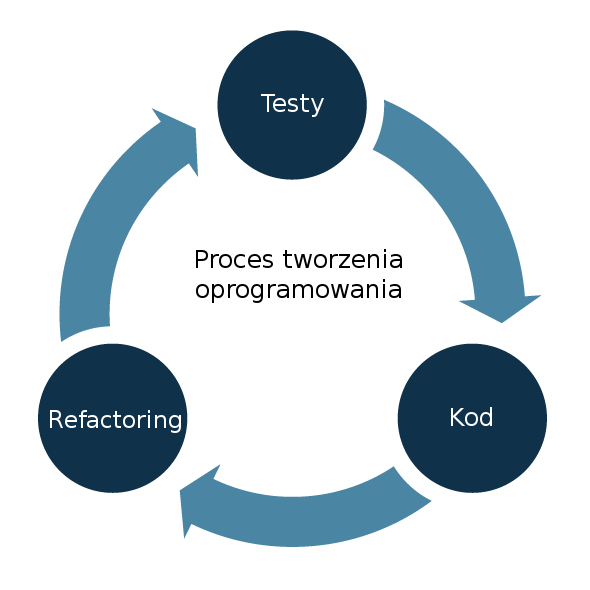
\includegraphics[scale=0.45]{images/test_cycle.png}
    \caption{Proces tworzenia oprogramowania}
	\end{figure}

	\newpage
  \subsection{Testy integracyjne}
  \subsection{Testy jednostkowe}
